\chapter{Possible Approaches \label{sec:PossibleApproaches}}

Veritest represents another tool that the developers of GraalVM could use to provide a \emph{certificate} for their implementation of optimization rules. 
To assist in verifying the optimization rule, the tool would need to be able to classify each of the optimization rules 
(See Fig. \ref{fig:classification}). Furthermore, there are several key non-functional requirements for the system that need to be satisfied 
(See Fig. \ref{fig:requirements}).

\begin{figure}[!htb]
      \begin{tabular}{|L{0.95\textwidth}|}
            \hline
            \begin{enumerate}
                  \item The optimization rule is false;
                  
                        This would require the tool to generate obvious counterexamples via Quickcheck (See \ref{sec:Quickcheck}) or Nitpick 
                        (See \ref{sec:Nitpick}).
              
                  \item The optimization rule is true;
                  
                        This would require the tool to verify that Sledgehammer (See \ref{sec:Quickcheck}) can provide proof obligations for the 
                        optimization rule \textbf{without} dynamically defining proof tactics.
              
                  \item The optimization rule would require manual proving by \emph{"proof experts"}.
                        
                        This means that the optimization is non-trivial: Isabelle is not able to find an obvious counterexample, and proving would require 
                        additional tactics or sub-goals to be defined.
            \end{enumerate} \\
            \hline
      \end{tabular}
      \caption{The classification of an optimization rule}
      \label{fig:classification}
\end{figure}

\begin{figure}[!htb]
      \begin{tabular}{|L{0.95\textwidth}|}
            \hline
            \begin{enumerate}
                  \item Developers of GraalVM need to be able to integrate this easily into their test suite;
                  \item Developers of GraalVM can easily use this without understanding Isabelle;
                  \item \emph{If possible}, the system doesn't require enormous computing resources locally.
            \end{enumerate} \\
            \hline
      \end{tabular}
      \caption{Non-functional requirements of the Framework}
      \label{fig:requirements}
\end{figure}

Understanding Isabelle's implementation is crucial to realize the goals of this project. At a glance, there are four possible approaches 
to the project:

\begin{itemize}
    \item Utilize Isabelle Client - Server interactions (See Sec. \ref{sec:IsabelleServer});
    \item Extend Isabelle/Scala (See Sec. \ref{sec:IsabelleScala});
    \item Utilize Isabelle CLI (See Sec. \ref{sec:IsabelleCLI})
    \item Create an Interpreter for GraalVM's optimization DSL (See Sec. \ref{sec:DSLInterpreter}).
\end{itemize}

\begin{figure}[!htb]
      \centering
      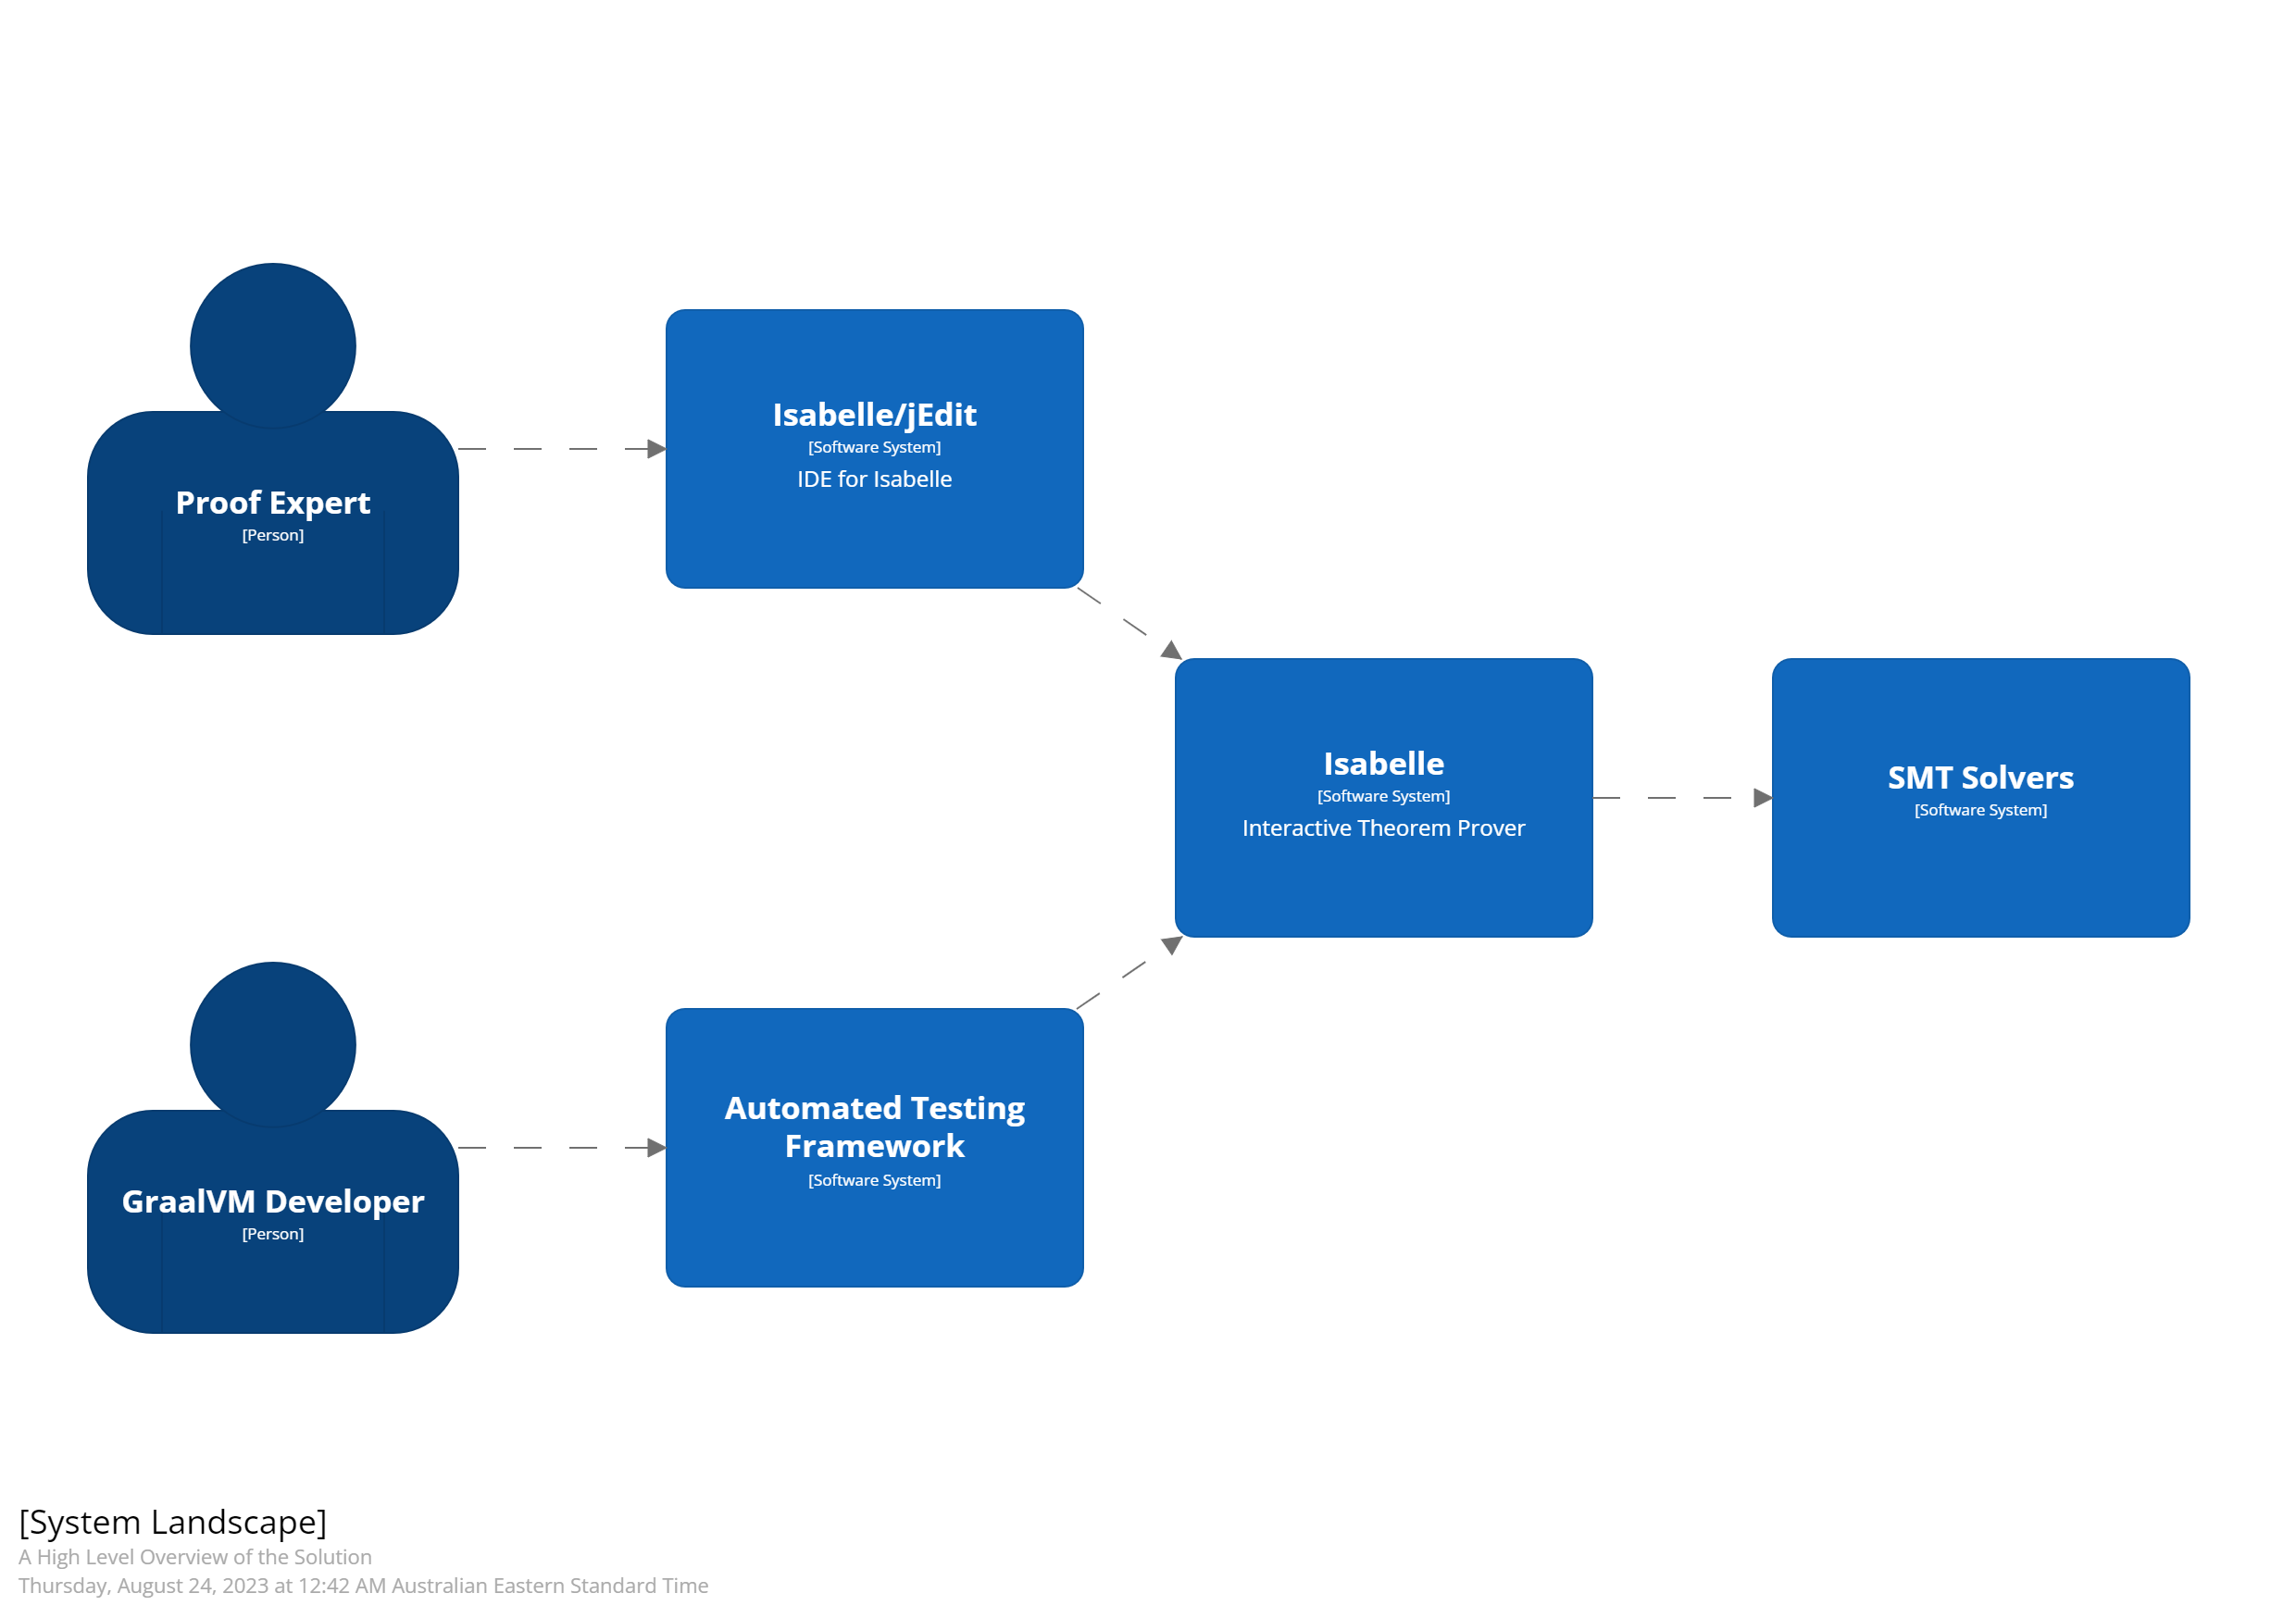
\includegraphics[width=1\textwidth]{structurizr-1-framework_overview_1.png}
      \caption{Proposed Solution}
      \label{fig:SystemLandscape}
\end{figure}

\todo[inline]{change veritest label from figure}

Fig. \ref{fig:SystemLandscape} depicts the overview of the proposed solution's system landscape. In theory, it would utilize Isabelle in a similar 
manner as Isabelle/jEdit \cite{isabelleSystem}. Therefore, it should be able to use the same Isabelle functionalities as Isabelle/jEdit does.

\section{Isabelle System Overview}
\label{sec:IsabelleSystemOverview}

\begin{figure}[!htb]
      \centering
      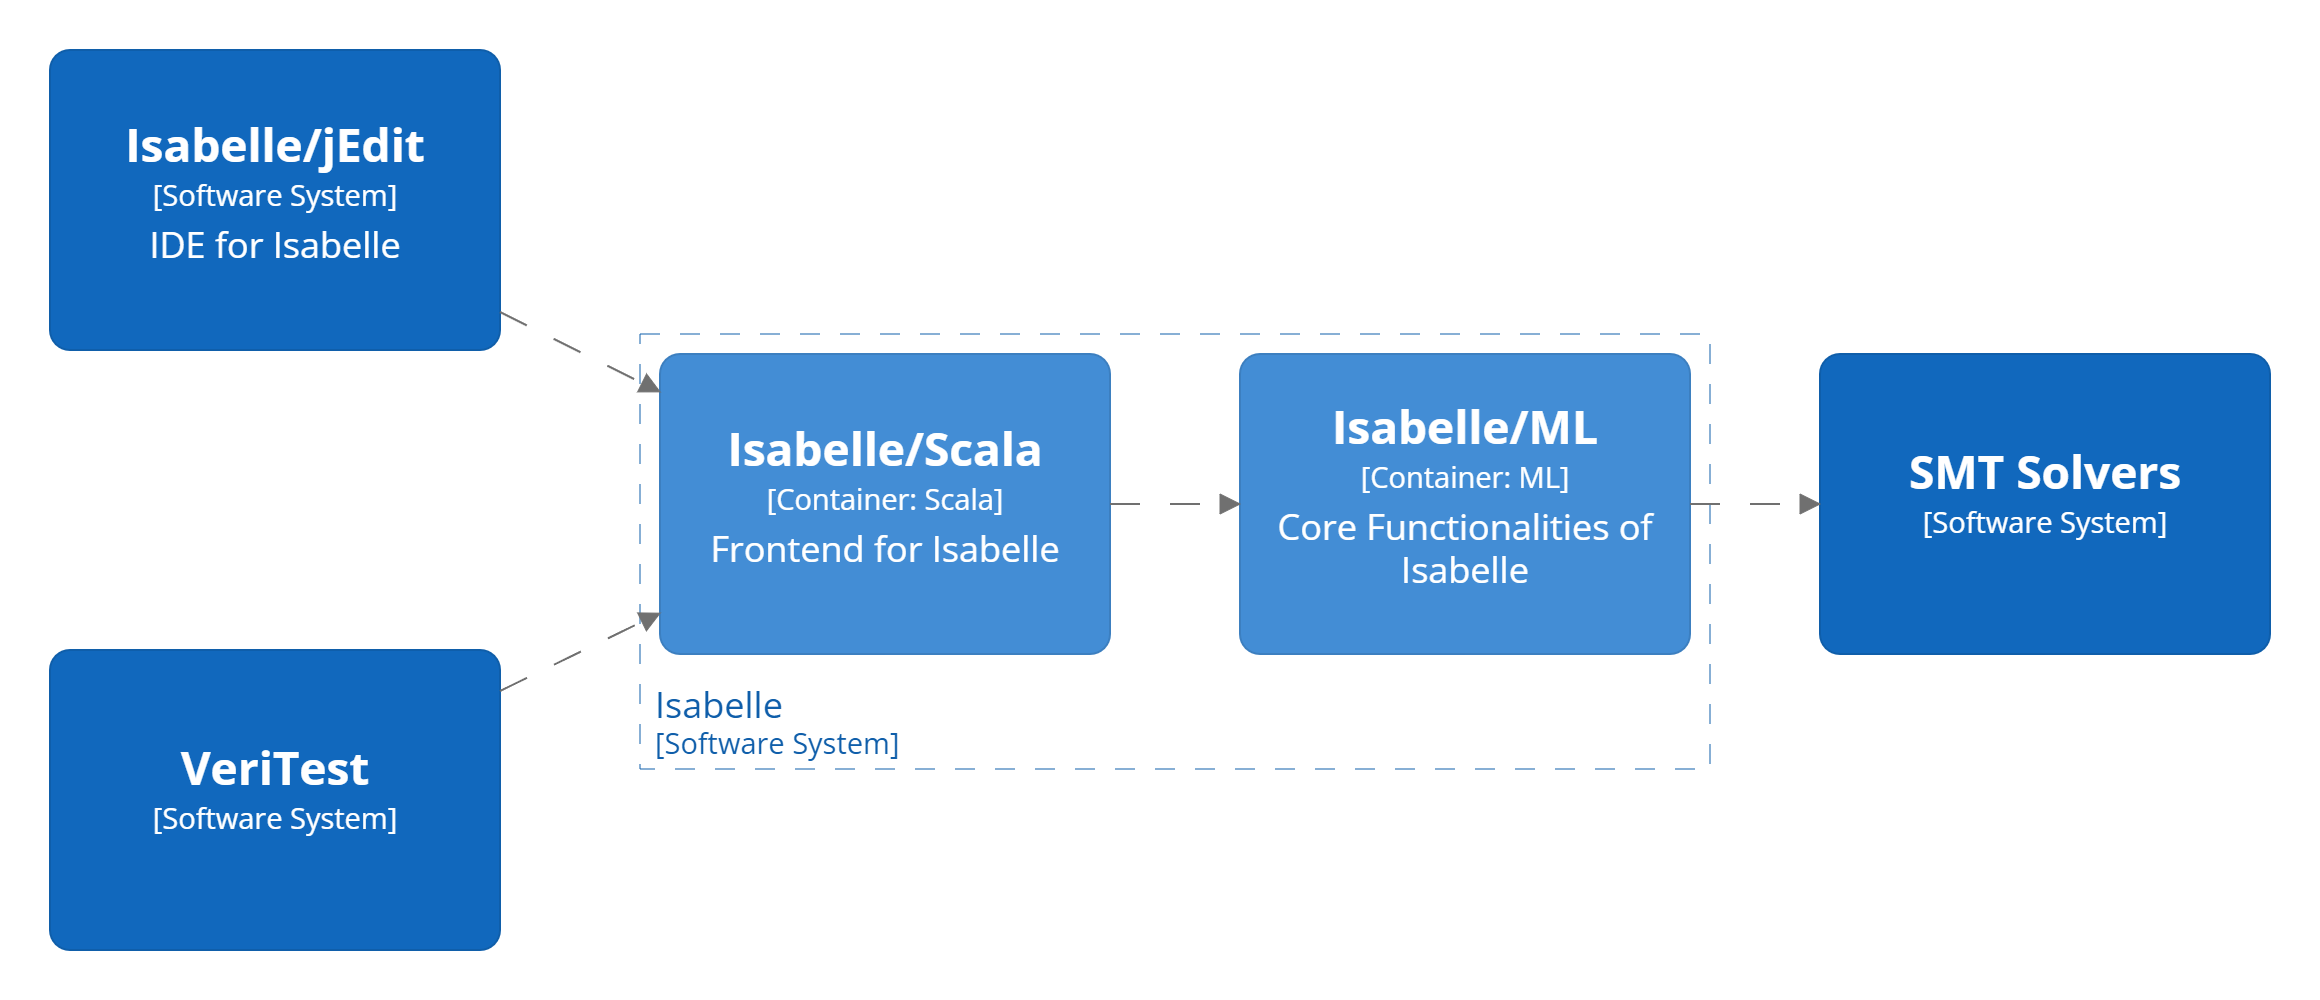
\includegraphics[width=1\textwidth]{structurizr-1-isabelle_overview_1.png}
      \caption{Isabelle System Overview}
      \label{fig:IsabelleSystem}
\end{figure}

Isabelle is made up of two significant components: Isabelle/ML and Isabelle/Scala \cite[Ch. 5]{isabelleSystem} (See Fig. \ref{fig:IsabelleSystem}). 
Isabelle/ML acts as the core functionality of Isabelle, harboring all the tools needed for proving theorems. Isabelle/Scala acts as the system 
infrastructure for Isabelle/ML -- hiding all implementation details of Isabelle/ML.

\section{Utilizing Isabelle Server}
\label{sec:IsabelleServer}

\begin{figure}[!htb]
      \centering
      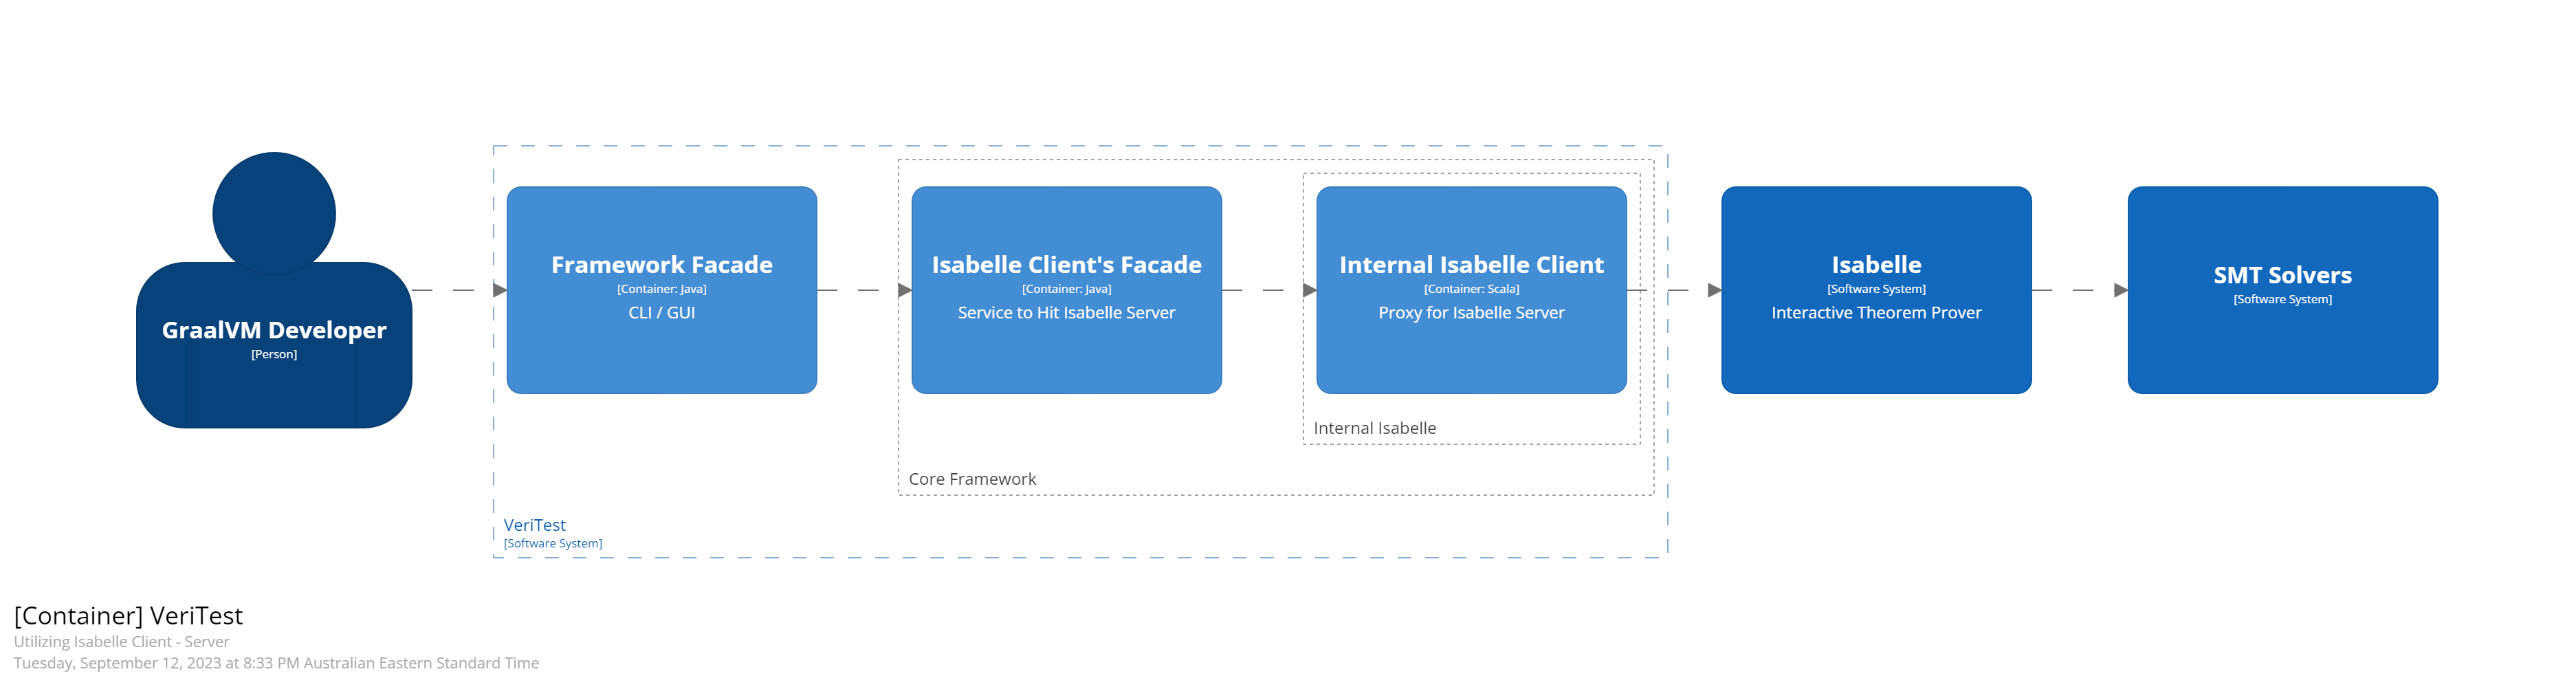
\includegraphics[width=1\textwidth]{structurizr-1-isabelle_client_server_1.png}
      \caption{Utilizing Isabelle Client - Server interaction}
      \label{fig:IsabelleServer}
\end{figure}

Isabelle Server acts as the core Isabelle process that allows theorems and all the required facts to be loaded up and processed by Isabelle/ML
\cite[Ch. 4]{isabelleSystem}. Interactions to Isabelle/Server would require a duplex socket connection over TCP \cite[Sec. 4.2]{isabelleSystem}. 
To simplify the communication between the framework and Isabelle/Server, we utilize Isabelle Client \cite[Sec. 4.1.2]{isabelleSystem} -- a proxy 
for Isabelle/Server that handles all the communication protocols of Isabelle/Server (See Fig. \ref{fig:IsabelleServer}).

Isabelle Server can load theorems and process requests in parallel \cite[Sec. 4.2.6]{isabelleSystem}. This implies that it would require a 
\emph{facade} that implements a demultiplexer for asynchronous messages on Isabelle Client (See Fig. \ref{fig:IsabelleServer}). As such, this 
solution -- \emph{theoretically} -- it would allow the framework to offload the computing resources of loading 
and processing optimization proofs at external sites (See Ch. \ref{sec:discussion}). VeriTest currently implements this approach, which is 
elaborated in detail in Ch. \ref{sec:implementation}.

\section{Extending Isabelle/Scala}
\label{sec:IsabelleScala}

\begin{figure}[!htb]
      \centering
      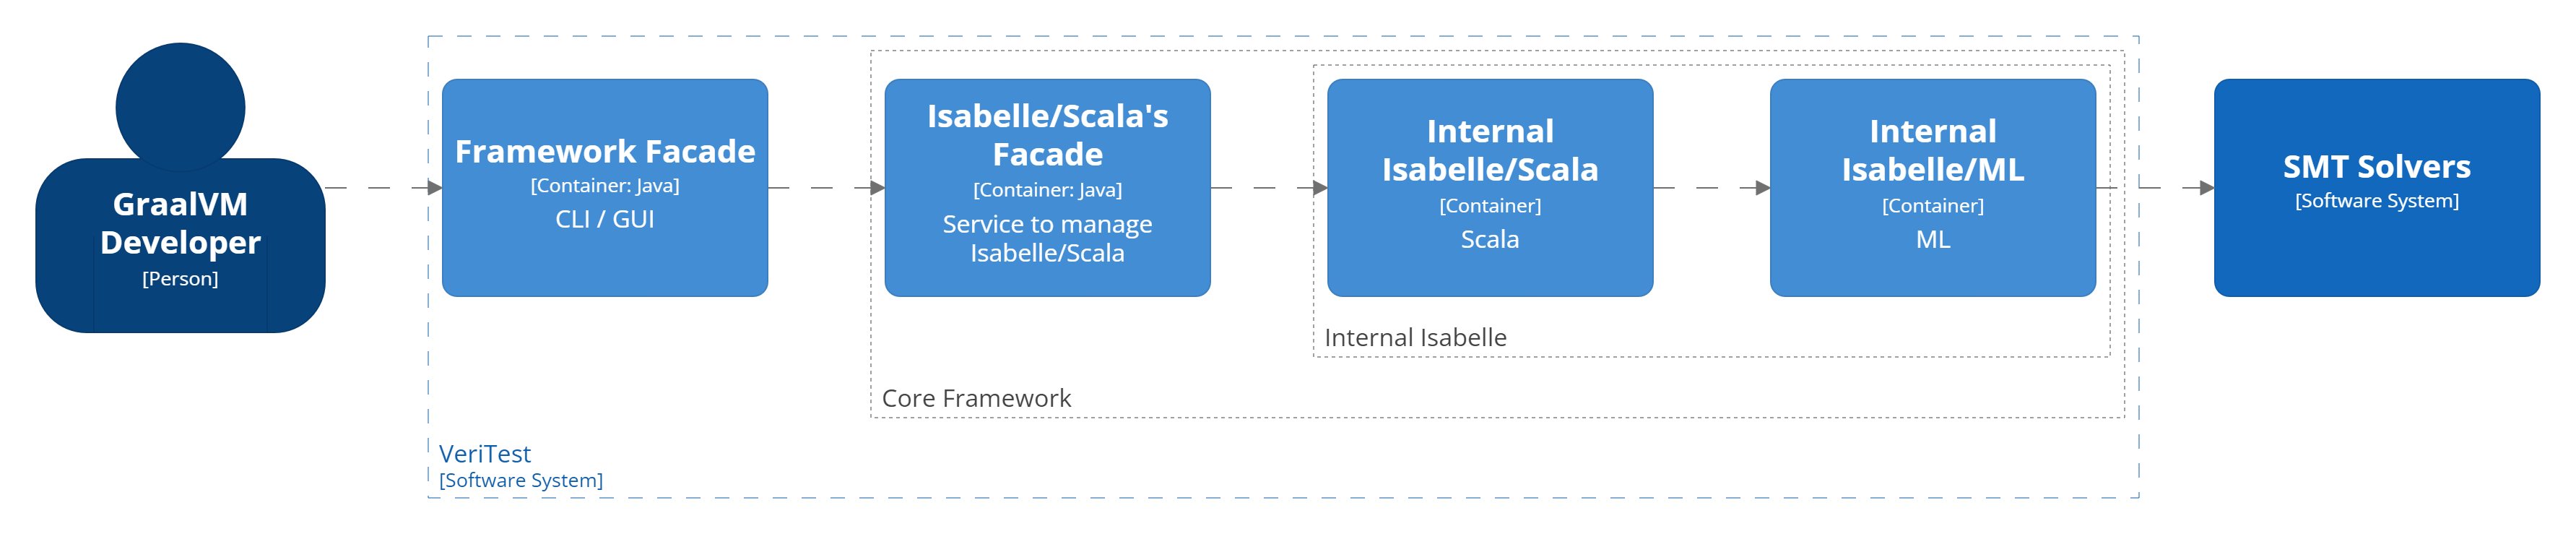
\includegraphics[width=1\textwidth]{structurizr-1-isabelle_scala_1.png}
      \caption{Extending Isabelle/Scala}
      \label{fig:IsabelleScala}
\end{figure}

Isabelle can be extended by accessing Isabelle/Scala functions \cite[Ch. 5]{isabelleSystem}. Extending Isabelle/Scala would require the framework 
to utilize Isablle's Scala compiler \cite[Sec. 5.1.4]{isabelleSystem}. Utilizing Isabelle/Scala would also mean that VeriTest would be capable of 
utilizing Isabelle/ML as well. Subsequently, this also implies that it is possible to extend and fine-tune existing automated tools to fit the 
requirements of this project. Fig. \ref{fig:IsabelleScala} depicts the proposed solution for this option.

However, the sheer complexity of Isabelle implies that extending Isabelle/Scala would require much of the 
project's timeline to understand Isabelle/Scala, which the time constraints of this thesis project does not allow. 
Furthermore, extending Isabelle/Scala \emph{could} mean that the framework would take up much of the computing resources to execute 
Isabelle/ML functions locally.

\section{Utilizing Isabelle CLI}
\label{sec:IsabelleCLI}

Veriopt's current semi-automated approach \cite[Sec. 5.1]{Term_Graph_Optimizations} utilizes Isabelle CLI, a wrapper for Isabelle/Scala functions 
\cite{IsabelleHOL}. As such, this solution would represent an Isabelle management service, where each optimization rule will be passed into an 
Isabelle/Scala function inside an Isabelle process and managed accordingly. In essence, the solution is similar to Sec. \ref{sec:IsabelleScala}. 
However, the solution will require additional processing overhead in the form of multiple local Isabelle processes for each of the optimization rules, 
instead of a single VeriTest and Isabelle instance.

\section{Interpreter for DSL}
\label{sec:DSLInterpreter}

Building an interpreter for GraalVM's optimization DSL acts as a last resort to the project. To implement this, it would require a significant 
amount of time to rework the DSL into the framework, and designing tools similar to Quickcheck (See Sec. \ref{sec:Quickcheck}) in order to satisfy the 
system requirements. Reinventing the wheel would not be productive for the project, and it would result in a tool that is far inferior to Isabelle.
Therefore, this option should be avoided.
